\section{Introduction}


\subsection{Articles}
\begin{frame}{Articles}
    \leftmargini=0pt
    \begin{itemize}
        \item \textbf{(2008) Fab-map: Probabilistic localization and mapping in the space of appearance}~\cite{fabmap2008b} ;
        \item (2009) Accelerating fab-map with concentration inequalities~\cite{accelerating} ;
        \item (2010) Fab-map 3d : Topological mapping with spatial and visual appearance~\cite{fabmap3d} ;
        \item \textbf{(2011) Appearance-only slam at large scale with fab-map~2.0}~\cite{fabmap2011} ;
        \item \textbf{(2012) Openfabmap : An open source toolbox for appearance-based loop closure detection}~\cite{openfabmap}.
    \end{itemize}
    \note[item]{Context ... Long sequences of FAB-MAP related articles...}
    \note[item]{Article getting OLD -- 2008, but...}
    \note[item]{For 1.0 and 2.0 Conference version first, then version journal}
    \note[item]{Non exaustive list... I might forget some}
\end{frame}

\subsection{FAB-MAP}
\begin{frame}{Fast Appearance-Based Mapping (FAB-MAP)}
    \begin{quotation}
        This paper describes a \textbf{probabilistic approach} to the problem of \textbf{recognizing places} based on their \textbf{appearance}. The system we present is not limited to localization, but \textbf{can determine that a new observation comes from a previously unseen place}, and so augment its map. Effectively this is a \textbf{SLAM} system in the space of appearance.~\cite{fabmap2008b}
    \end{quotation}
    \note[item]{Read it first}
    \note[item]{Place recognition}
    \note[item]{Appearance, using visual features from camera as oposed to geometrical features}
    \note[item]{New observation != simple nearest neighbour}
    \note[item]{SLAM ? I'll let you decide}
\end{frame}

\subsection{Basic concepts}
\begin{frame}{Map: Metric vs Topological}
    \begin{figure}
        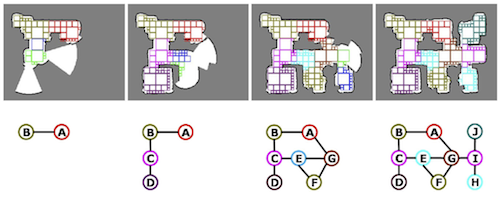
\includegraphics[width=1.0\textwidth]{./media/metric_vs_topo.png}
        \caption{Source: http://www.autonomousrobotsblog.com/}
    \end{figure}
    \note[item]{Metric (distance between all members)}
    \note[item]{Topological (set of points, along with a set of neighbourhoods for each point)}
    \note[item]{There is mathematical definition available if you prefer...}
\end{frame}

\begin{frame}{Simultaneous Localization And Mapping (SLAM)}
    \begin{center}
        \href{https://www.youtube.com/watch?v=y7OnimZRj2w}{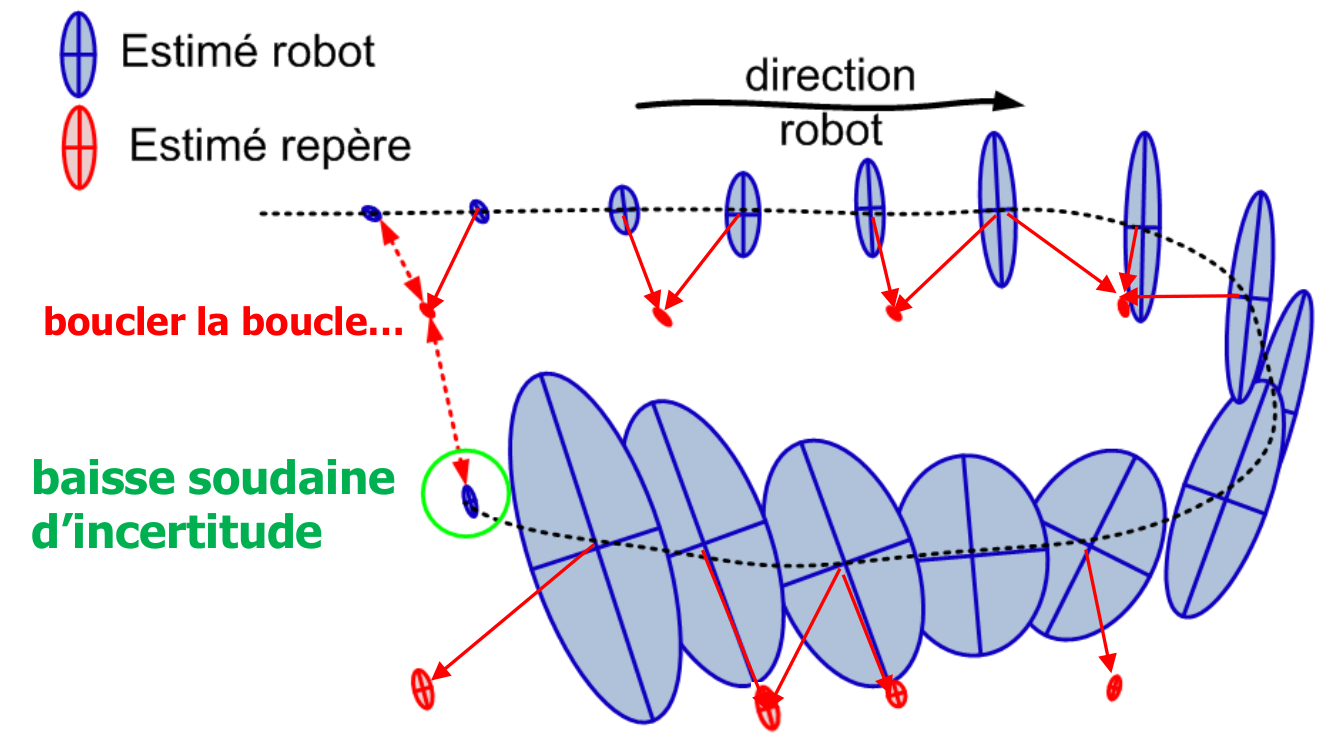
\includegraphics[width=1.0\textwidth]{./media/loop_closure.png}}
    \end{center}
    \note[item]{SLAM demo... Find points, update map...}
    \note[item]{Place recognition (what and why)}
    \note[item]{Loop closure}
    \note[item]{How is it related to FAB-MAP: topological loop closure}
\end{frame}
